
\begin{figure*}[tbp]
\begin{center}
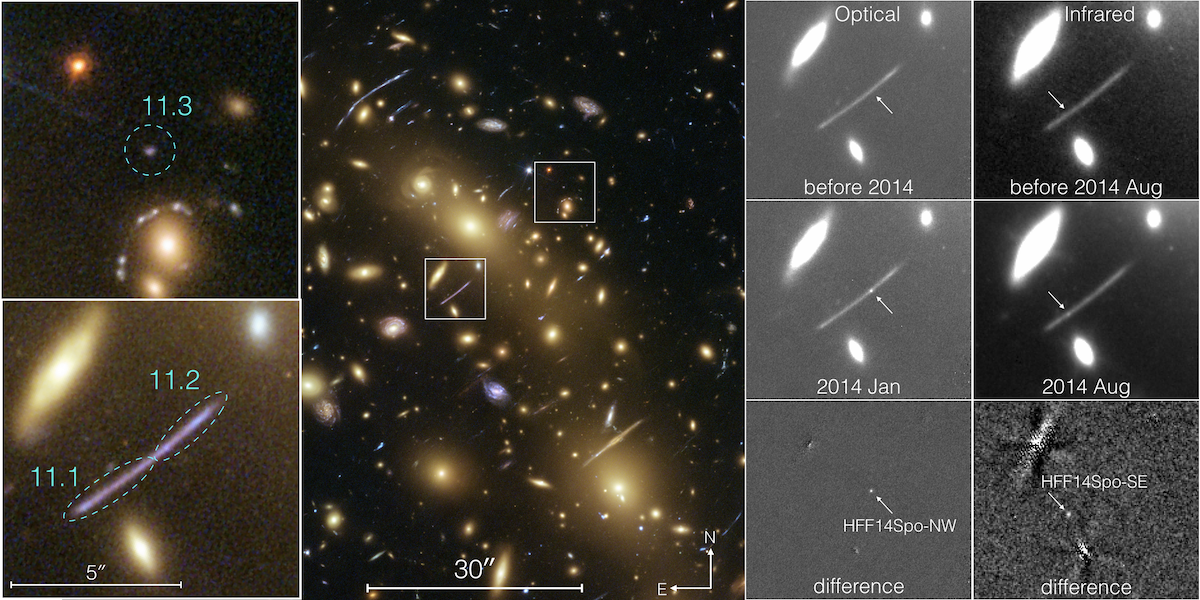
\includegraphics[width=1\textwidth]{./figures/detection_image/detection_image.png}
\caption{ \protect\label{fig:SpockDetectionImages}
The detection of \spockone and \spocktwo in \HST imaging from the
Hubble Frontier Fields. The central panel shows the full field of the
MACSJ0416 cluster, in a combined image using optical and infrared
bands from \HST.  Two boxes within the main panel demarcate the regions
where the \spock host-galaxy images appear. These regions are shown as
two inset panels on the left, highlighting the three images of the
host galaxy (labeled 11.1, 11.2, and 11.3), which are caused by the
gravitational lensing of the cluster.  Two columns on the right side
show the discovery of the two transient events in optical and infrared
light, respectively.  In these final two columns the top row is a
template image, the center row shows the epoch when each transient
appeared, and the bottom row is the difference image.
}
\end{center}
\end{figure*}

%\end{multicols}
\begin{deluxetable}{lccccc}
  \tablewidth{0.7\textwidth}
  \tablecolumns{6}
  \tablecaption{Lens model predictions for time delays and
    magnifications at the observed locations of the \spock
    transients. \label{tab:LensModelPredictions}}
  \tablehead{
    \colhead{Model} &
    \colhead{$\lvert\mu_{\rm NW}\rvert$} & \colhead{$\lvert\mu_{\rm SE}\rvert$} &
    \colhead{$\lvert\mu_{11.3}\rvert$} &  
    \colhead{$\Delta t_{\rm NW:SE}$} & \colhead{$\Delta t_{\rm NW:11.3}$} \\
    \colhead{} & \colhead{} & \colhead{} & \colhead{} & \colhead{(days)} & \colhead{(years)}}
\startdata
CATS &  196$^{+140}_{-53}$ & 46$^{+2}_{-1}$ & 3.3$^{+0.0}_{-0.0}$ & -1.7$^{+2.0}_{-1.9}$ & -3.7$^{+0.1}_{-0.2}$\\[0.5em]
GLAFIC & 29$^{+43}_{-10}$ &  84$^{+103}_{-38}$ &  3.0$^{+0.2}_{-0.2}$ &  4.1$^{+5.5}_{-3.4}$ &  -5.0$^{+0.5}_{-0.6}$\\[0.5em]
GLEE & 182$^{+203}_{-83}$ &  67$^{+31}_{-16}$ &  2.9$^{+0.1}_{-0.1}$ &  36$^{+6}_{-7}$ &  -6.1$^{+0.3}_{-0.2}$\\[0.5em]
GRALE & 13$^{+11}_{-6}$ & 12$^{+9}_{-5}$ & 3.1$^{+2.2}_{-0.9}$ & -10$^{+1}_{-7}$ & -2.5$^{+1.0}_{-3.1}$ \\[0.5em]
SWunited & 38$\pm8$ & 13$\pm1$ & 2.9 $\pm0.1$ & \nodata & \nodata \\[0.5em]
WSLAP$^{+}$ & 35$\pm$20 & 30$\pm$20 & \nodata & -48$\pm$10 & 0.8  \\[0.5em]
ZLTM & 103$^{+48}_{-40}$ & 32$^{+8}_{-10}$ & 3.5$\pm$0.3  & 43$^{+12}_{-10}$ & -3.7$\pm0.3$\\
\enddata
\tablecomments{ Each lens model is identified by the name of the
  modeling team or tool. Time delays give the predicted delay relative
  to an appearance in the NW host image, 11.2. Positive (negative)
  values indicate the NW image is the leading (trailing) image of the
  pair.  The observed time lag between the NW and SE events was
  $\Delta t_{\rm NW:SE}=234\pm6$ days.}
  \label{tab:LensModelPredictions}
\end{deluxetable}

%\begin{multicols}{2}

\begin{figure*}[tbp]
  \begin{center}
    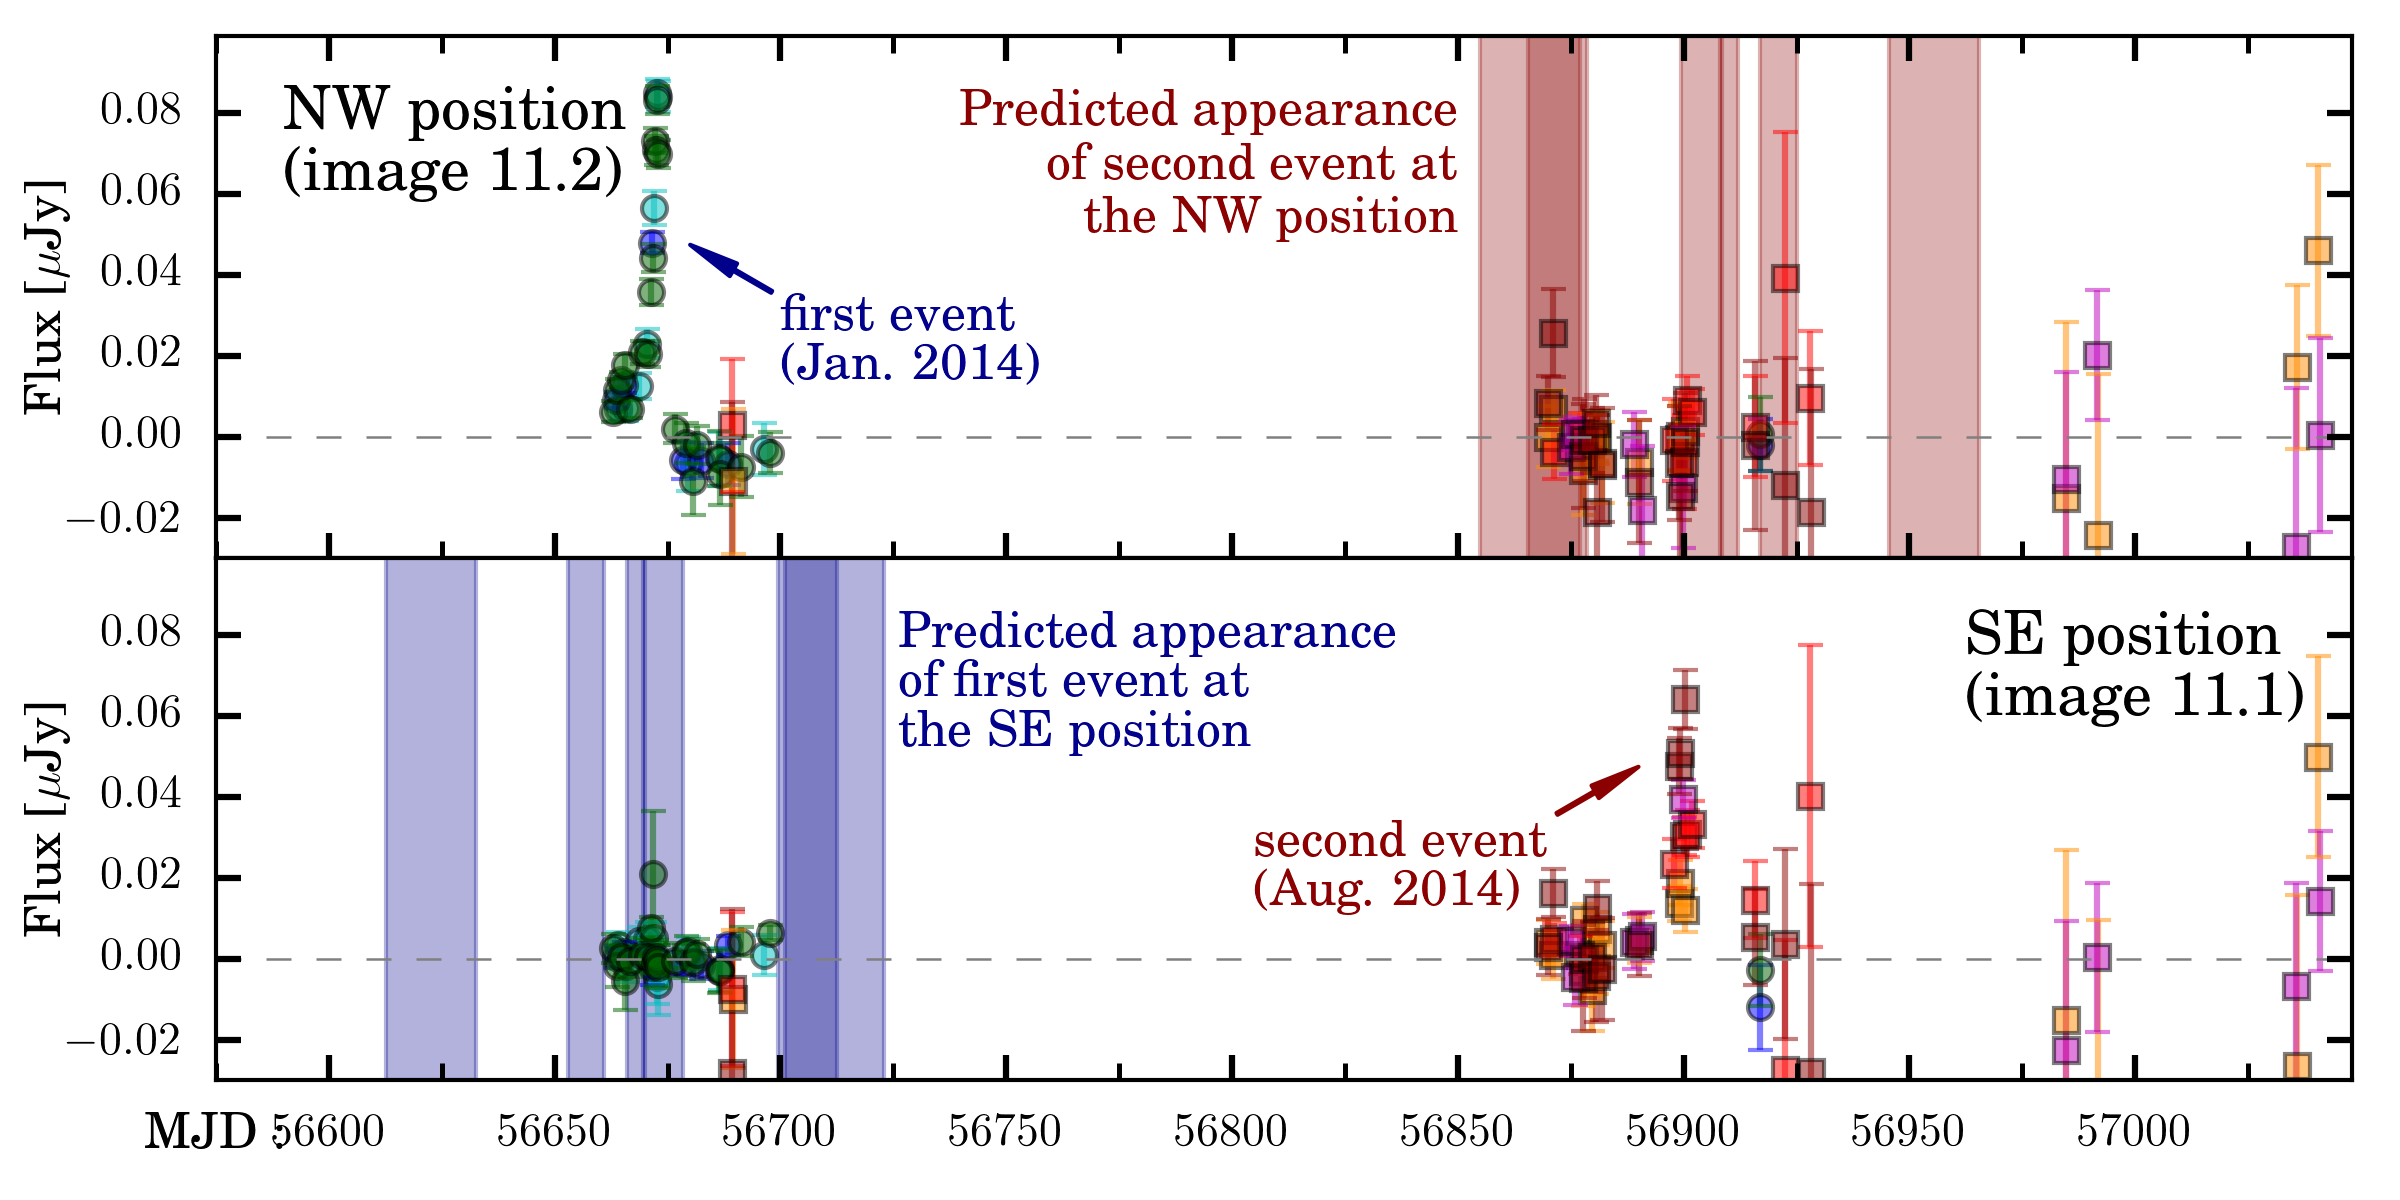
\includegraphics[width=\textwidth]{./figures/spock_predictions/spock_predictions}
    \caption{\protect\label{fig:SpockDelayPredictions}
Predictions for the reappearance episodes of both \spockone
and \spocktwo due to gravitational lensing time delays, as listed in
Table~\ref{tab:LensModelPredictions}.  The top panel shows photometry
collected at the NW position (host galaxy image 11.2) where the first
event (\spockone, labeled Spock-1) appeared in January, 2014.  Optical
measurements from ACS are in blue and green, and infrared observations
from WFC3-IR are in red and orange, as in
Figure~\ref{fig:LightCurves}.  Each blue bar in the lower panel shows
one lens model prediction for the dates when that same physical event
(\spockone) would have also appeared in the SE location (galaxy image
11.1), due to gravitational lensing time delay.  The lower panel plots
photometry from the SE position (11.1). On the right side we see the
second observed event (\spocktwo, labeled Spock-2).  The red bars above
show model predictions for when the NW host image 11.2 would have
exhibited the gravitationally delayed image of the \spocktwo\ event.
The width of each bar encompasses the 68\% confidence region for a
single model, and darker regions indicate an overlap from multiple
models.
  
}
  \end{center}
\end{figure*}


\begin{figure*}[tbp]
  \begin{center}
    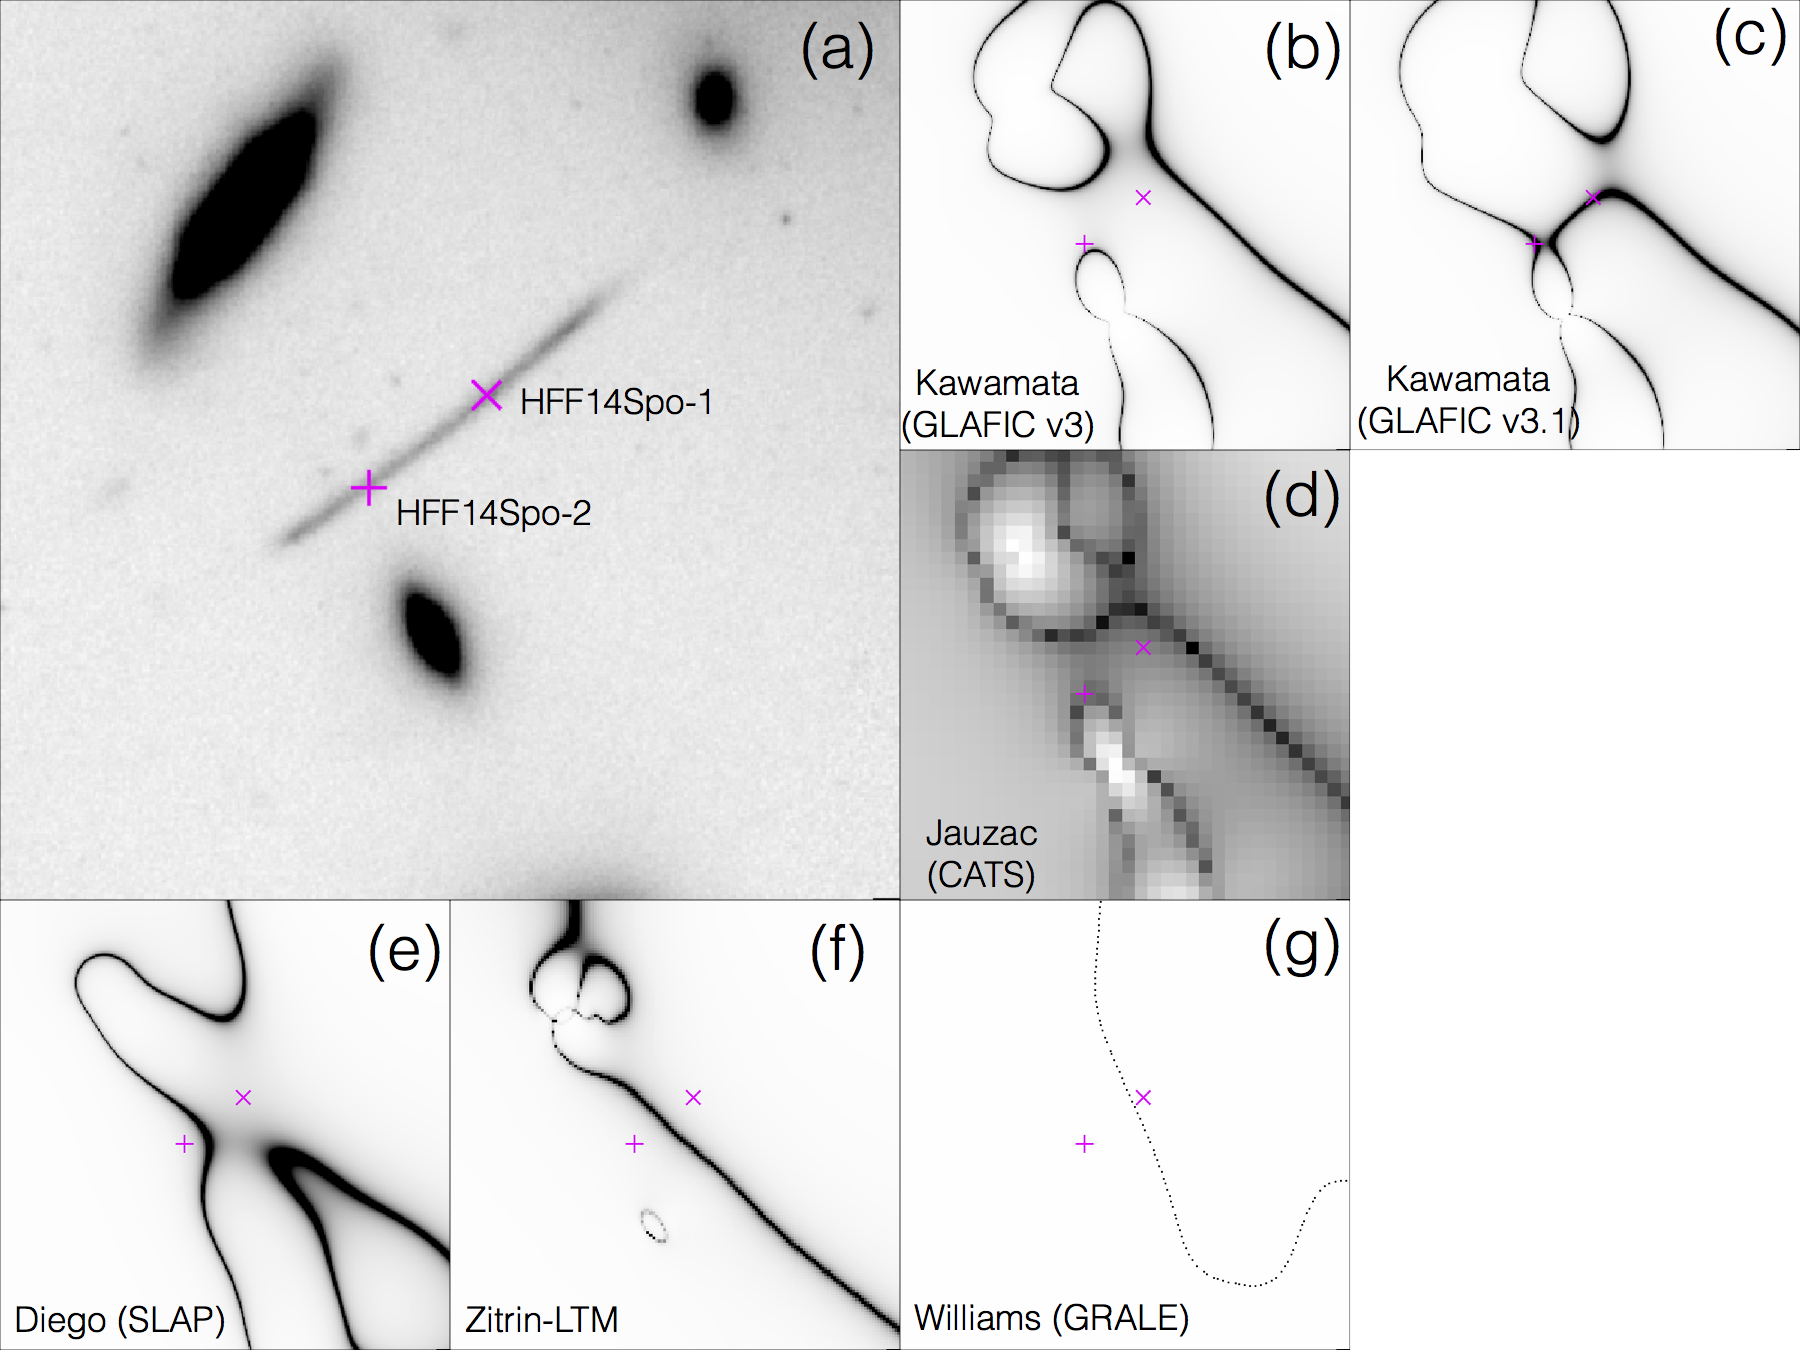
\includegraphics[width=\textwidth]{./figures/spock_critical_curves/spock_critical_curves.png}
    \caption{\protect\label{fig:SpockCriticalCurves}
Locations of the lensing critical curves relative to the positions of
the two \spock sources. Panel (a) marks the \spock locations on the
HST Frontier Fields image of the MACS0416 field in the F814W (I) band.
Panels b-f show magnification maps derived from the Kawamata, Jauzac,
Diego and Zitrin lens models.  All are scaled so that white is $\mu=1$
and black indicates $\mu=1000$.  Panel (g) depicts a trace of the
lensing critical curve near the \spock positions from the GRALE
model. The models shown in b, c and d have separate critical curves
passing near to the two \spock positions. Models in e, f and g have a
single critical curve passing between the two transient locations.
The GLAFIC v3.1 model shown in (c) was defined with the requirement
that multiple critical curves pass through the \spock locations.  All
other panels present the model realization that provides the best fit
to the lensing constraints.}
  \end{center}
\end{figure*}

\begin{figure*}[tbp]
\begin{center}
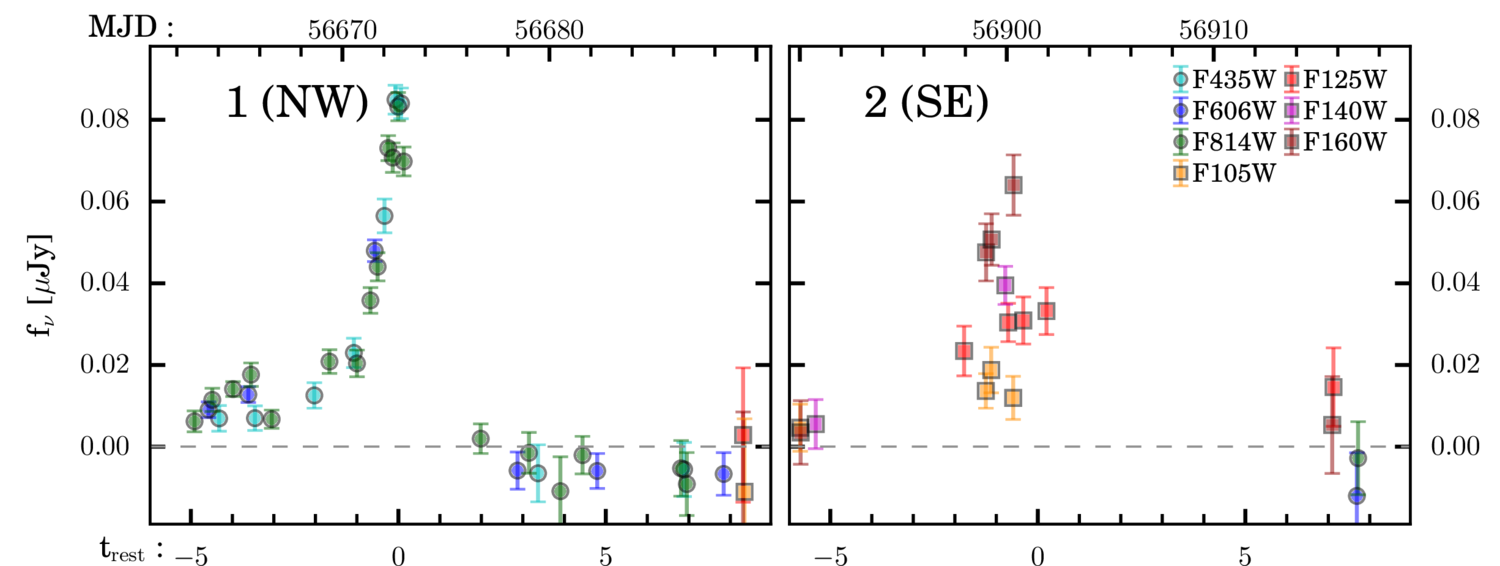
\includegraphics[width=1\textwidth]{./figures/spock_lightcurves/spock_lightcurves_flux}
\caption{ \protect\label{fig:LightCurves}
Light curves for the two transient events, \spockone\ on the left
and \spocktwo\ on the right.  Measured fluxes in micro-Janskys are
plotted against rest-frame time at $z=1.0054$, relative to the time of
the peak observed flux for each event. The corresponding Modified
Julian Date (MJD) in the observer frame is marked on the top axis for
each panel.  As indicated in the legend, optical observations using
the \HST\ ACS-WFC detector are plotted as circles, while infrared
measurements from the WFC3-IR detector are plotted as squares.

  
}
\end{center}
\end{figure*}


\begin{figure*}[tbp]
\begin{center}
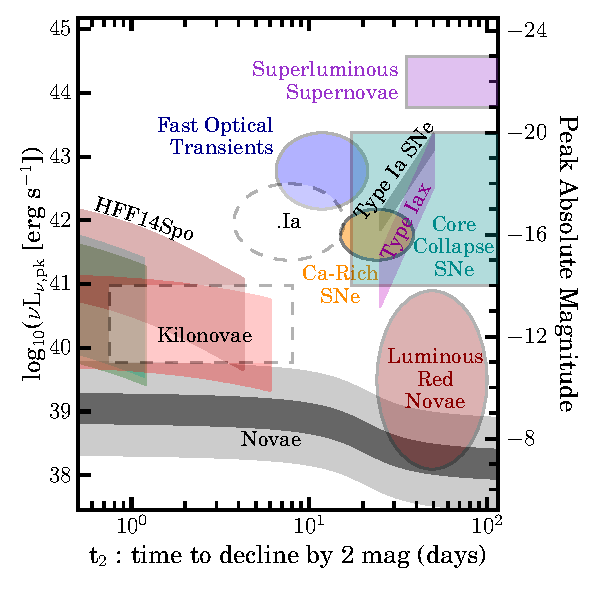
\includegraphics[width=0.48\textwidth]{./figures/peakluminosity_vs_declinetime/peakluminosity_vs_declinetime_sn}
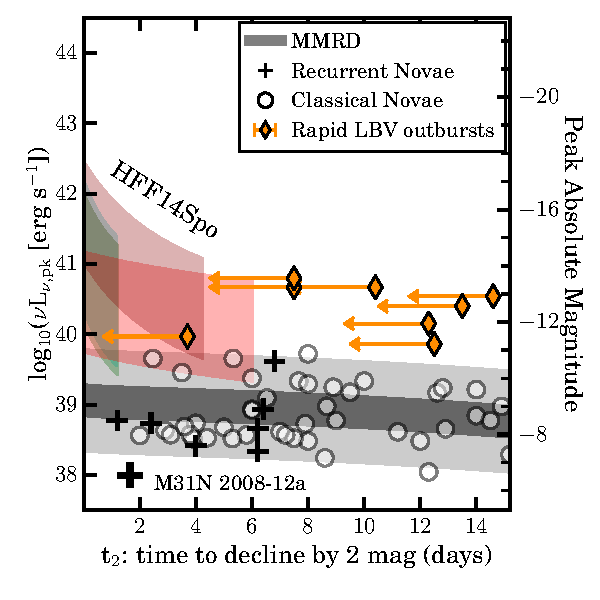
\includegraphics[width=0.48\textwidth]{./figures/peakluminosity_vs_declinetime/peakluminosity_vs_declinetime_nova_lbv}
\caption{ \protect\label{fig:PeakLuminosityDeclineTime}
Peak luminosity vs. decline time for \spock and assorted categories of
explosive transients.  Observed constraints of the \spock events are
plotted as overlapping colored bands, along the left side of the
figure.  \spockone is shown as cyan and blue bands, corresponding to
independent constraints drawn from the F435W and F814W light curves,
respectively.  For \spocktwo the scarlet and maroon bands show
constraints from the F125W and F160W light curves, respectively.  The
width and height of these bands incorporates the uncertainty due to
magnification (we adopt $7<\mu_{\rm NW}<485$ and $7<\mu_{\rm SE}<185$; see Table ~\ref{tab:LensModelPredictions}) and the time of peak.  In
the top panel, ellipses and rectangles mark the luminosity and
decline-time regions occupied by various explosive transient classes.
Filled shapes show the empirical bounds for transients with a
substantial sample of known events. Dashed regions mark theoretical
expectations for rare transients that lack a significant sample size:
the ``.Ia'' class of white dwarf He shell detonations and the kilonova
class from neutron star mergers.  Grey bands in both panels show the
MMRD relation for classical novae.  In the lower panel, circles mark
the observed peak luminosities and decline times for classical novae,
while black `+' symbols mark recurrent novae from our own galaxy.  The
large cross labeled at the bottom shows the rapid recurrence nova M31N
2008-12a.  Each orange diamond marks a separate short transient event
from the two rapid LBV outburst systems, SN
2009ip \citep{Pastorello:2013} and NGC3432-LBV1 \citep[a.k.a. SN
2000ch][]{Pastorello:2010}.  These LBV events provide only upper
limits on the decline time due to limited photometric sampling.
}
\end{center}
\end{figure*}


